\documentclass[a4paper,12pt]{article}
\usepackage{geometry}
\geometry{margin=1in}
\usepackage{graphicx}
\usepackage{amsmath, amssymb, amsthm}
\usepackage{fancyhdr}
\usepackage{xcolor}
\usepackage{hyperref}
\usepackage{tikz}
\usepackage{circuitikz}
\usepackage{minted}
% Header and Footer Style
\pagestyle{fancy}
\fancyhf{}
\rhead{\textbf{Assignment-01}}
\lhead{Engineering Electromagnetics}
\cfoot{\thepage}

% Title Page
\begin{document}
\begin{titlepage}
    \centering
    {\Huge \textbf{ASSIGNMENT-01}}\\[1cm]
    {\Large EE1204}\\[1.5cm]
    \rule{\linewidth}{0.5mm} \\[0.4cm]
    {\Huge \textbf{ENGINEERING ELECTROMAGNETICS}}\\[0.4cm]
    \rule{\linewidth}{0.5mm} \\[1.5cm]
    
    \textbf{Submitted by:}\\
    {Krishna Hanumanth Patil}\\
    {IIT Hyderabad}\\
    {EE24BTECH11036}\\[1cm]
    \textbf{Submitted to:}\\
    {Prof. Aneesh S}\\[1.5cm]
    
    \vfill
    \textbf{\today}\\
    \vfill
\end{titlepage}

% Problem-01
\section{Two points charges of equal magnitude $q$ are positioned at $z=\pm \frac{d}{2}$. Determine:}
\subsection{The electric field everywhere on the z-axis.}
\textbf{Solution :} Below is the diagram for the question:

\begin{figure}[!ht]
\centering
\resizebox{0.6\textwidth}{!}{%
\begin{circuitikz}
\tikzset{every node/.style={font=\normalsize}}
\draw [<->, >=Stealth] (8.75,17.25) -- (8.75,5.75);
\draw [<->, >=Stealth] (6.5,11) -- (15.25,11);
\node at (8.75,13.5) [circ] {};
\node at (8.75,8.5) [circ] {};
\node [font=\small] at (8.25,13.75) {A};
\node [font=\small] at (8.25,8.75) {B};
\node [font=\small] at (9.25,13.5) {+q};
\node [font=\small] at (9.25,8.5) {-q}; % Fix charge sign for clarity
\node at (8.75,15.25) [circ] {};
\draw [<->, >=Stealth] (10,15.25) -- (10,11) node[pos=0.5, fill=white]{$z$}; % Removed undefined
\draw [<->, >=Stealth] (7.75,11) -- (7.75,13.5) node[pos=0.5, fill=white]{$d/2$};
\draw [<->, >=Stealth] (7.75,11) -- (7.75,8.5) node[pos=0.5, fill=white]{$d/2$};
\node [font=\small] at (8.25,15.25) {P};
\draw [line width=0.9pt, ->, >=Stealth] (8.75,15.25) -- (8.75,16.5);
\draw [color={rgb,255:red,145; green,29; blue,29}, line width=0.9pt, ->, >=Stealth] (8.75,15.25) -- (8.75,16.5);
\node [font=\small, color={rgb,255:red,145; green,29; blue,29}] at (8,16.25) {$E_{PA}$};
	\node [font=\small, color={rgb,255:red,23; green,23; blue,23}] at (9.25,16.25) {$E_{PB}$}; % Removed duplicate label
\node [font=\normalsize, color={rgb,255:red,23; green,23; blue,23}] at (9.25,17.5) {z-axis};
\node [font=\normalsize, color={rgb,255:red,23; green,23; blue,23}] at (15.25,10.75) {x-axis};
\end{circuitikz}
}
\label{fig:my_label}
\end{figure}

The position vectors for the points A,B,P are :
\begin{align}
	\vec{r_{A}} &= \frac{d}{2} \hat{k} \\
	\vec{r_{B}} &= -\frac{d}{2} \hat{k} \\
	\vec{r_{P}} &= x \hat{k}
\end{align}

The electric field at the point P due to a charge $q$ at point A is :
\begin{align}
	E_{PA} &= \frac{kq}{(|r_P - r_A|)^3}  \, \, (\vec{r_P} - \vec{r_A}) \\
	E_{PA} &= \frac{kq}{(x-\frac{d}{2})^3} \, \, (x-\frac{d}{2}) \hat{k} \\
	E_{PA} &= \frac{kq}{(x-\frac{d}{2})^2} \, \, \hat{k}
\end{align}
where $ k = \frac{1}{4\pi{{\epsilon}_0}} $ \\
Similiarly , the electric field at the point P due to a charge $q$ at the point B is :
\begin{align}
	E_{PB} &= \frac{kq}{(|r_P - r_B|)^3}  \, \, (\vec{r_P} - \vec{r_B}) \\
	E_{PB} &= \frac{kq}{(x+\frac{d}{2})^3} \, \, (x+\frac{d}{2}) \hat{k} \\
	E_{PB} &= \frac{kq}{(x+\frac{d}{2})^2} \, \, \hat{k}
\end{align}
Now, by Principle of superposition, 
\begin{align}
	E_P &= E_{PA} + E_{PB} \\
	    &= \frac{kq}{(x-\frac{d}{2})^2} \, \, \hat{k} + \frac{kq}{(x+\frac{d}{2})^2} \, \, \hat{k} \\
	    &= \boxed{\frac{kq(2x^2+\frac{d^2}{2})}{(x^2 - \frac{d^2}{4})^2} \, \, \hat{k}}
\end{align}

\subsection{The electric field everywhere on the x-axis.}
\textbf{Solution :} Below is the diagram for the question :
\begin{figure}[!ht]
\centering
\resizebox{0.6\textwidth}{!}{%
\begin{circuitikz}
\tikzstyle{every node}=[font=\normalsize]
\draw [<->, >=Stealth] (10,14.25) -- (10,4.25);
\draw [<->, >=Stealth] (7.5,9.25) -- (17.75,9.25);
\node at (10,11.75) [circ] {};
\node at (10,6.75) [circ] {};
\node at (15,9.25) [circ] {};
\draw [<->, >=Stealth] (10.25,8.75) -- (14.75,8.75)node[pos=0.5, fill=white]{x};
\draw [<->, >=Stealth] (10.25,11.75) -- (10.25,9.25)node[pos=0.5, fill=white]{d/2};
\draw [<->, >=Stealth] (10.25,9.25) -- (10.25,6.75)node[pos=0.5, fill=white]{d/2};
\node [font=\normalsize] at (9.25,11.75) {+q};
\node [font=\normalsize] at (9.25,6.75) {+q};
\node [font=\normalsize] at (9.75,12.25) {A};
\node [font=\normalsize] at (9.75,6.25) {B};
\node [font=\normalsize] at (15.25,8.75) {P};
\draw [->, >=Stealth] (15,9.25) -- (16.75,8)node[pos=0.5, fill=white]{$E_{PA}$};
\draw [->, >=Stealth] (15,9.25) -- (16.75,10.5)node[pos=0.5, fill=white]{$E_{PB}$};
\draw [color={rgb,255:red,36; green,204; blue,78}, ->, >=Stealth] (15,9.25) -- (16.75,9.25)node[pos=0.5, fill=white]{\textbf{$E_{P}$}};
\draw [dashed] (16.75,10.5) -- (16.75,8);
\node [font=\normalsize] at (17.75,9) {\textbf{x-axis}};
\node [font=\normalsize] at (10.25,14.5) {\textbf{z-axis}};
\end{circuitikz}
}%
\caption{Description of the circuit.} % Optional: Add a caption
\label{fig:my_label}
\end{figure}

The position vectors for the points \( A, B, P \) are:
\begin{align}
    \vec{r}_{A} &= \frac{d}{2} \hat{k} \\
    \vec{r}_{B} &= -\frac{d}{2} \hat{k} \\
    \vec{r}_{P} &= x \hat{i}
\end{align}

The electric field at the point \( P \) due to a charge \( q \) at point \( A \) is:
\begin{align}
    \vec{E}_{PA} &= \frac{kq}{|\vec{r}_P - \vec{r}_A|^3} (\vec{r}_P - \vec{r}_A) \\
    &= \frac{kq}{(x^2 + \frac{d^2}{4})^{3/2}} \left( x \hat{i} - \frac{d}{2} \hat{k} \right)
\end{align}

Similarly, the electric field at the point \( P \) due to a charge \( q \) at point \( B \) is:
\begin{align}
    \vec{E}_{PB} &= \frac{kq}{|\vec{r}_P - \vec{r}_B|^3} (\vec{r}_P - \vec{r}_B) \\
    &= \frac{kq}{(x^2 + \frac{d^2}{4})^{3/2}} \left( x \hat{i} + \frac{d}{2} \hat{k} \right)
\end{align}

Now, by the principle of superposition:
\begin{align}
    \vec{E}_P &= \vec{E}_{PA} + \vec{E}_{PB} \\
    &= \frac{kq}{(x^2 + \frac{d^2}{4})^{3/2}} \left( x \hat{i} - \frac{d}{2} \hat{k} \right) + \frac{kq}{(x^2 + \frac{d^2}{4})^{3/2}} \left( x \hat{i} + \frac{d}{2} \hat{k} \right) \\
    &= \frac{kq}{(x^2 + \frac{d^2}{4})^{3/2}} \left( 2x \hat{i} \right) \\
	&= \boxed{\frac{2kqx}{(x^2 + \frac{d^2}{4})^{3/2}} \hat{i}}
\end{align}

\subsection{Calculate the above for the above parts if the charge at $z = -\frac{d}{2}$ is $-q$ instead of $q$.}
\textbf{Solution :} \\ For part (a) : \\
The electric field at the point $P_z$ due to a charge $q$ at point A is:
\begin{align}
    E_{PA} &= \frac{kq}{(|r_P - r_A|)^3} (\vec{r_P} - \vec{r_A}) \\
    &= \frac{kq}{(x - \frac{d}{2})^3} (x - \frac{d}{2}) \hat{k} \\
    &= \frac{kq}{(x - \frac{d}{2})^2} \hat{k}
\end{align}
where $k = \frac{1}{4\pi{{\epsilon}_0}}$. \\

Similarly, the electric field at the point $P_z$ due to a charge $-q$ at point B is:
\begin{align}
    E_{PB} &= \frac{k(-q)}{(|r_P - r_B|)^3} (\vec{r_P} - \vec{r_B}) \\
    &= -\frac{kq}{(x + \frac{d}{2})^3} (x + \frac{d}{2}) \hat{k} \\
    &= -\frac{kq}{(x + \frac{d}{2})^2} \hat{k}
\end{align}

Now, by the principle of superposition:
\begin{align}
    E_P &= E_{PA} + E_{PB} \\
        &= \frac{kq}{(x - \frac{d}{2})^2} \hat{k} - \frac{kq}{(x + \frac{d}{2})^2} \hat{k} \\
        &= \left( \frac{kq}{(x - \frac{d}{2})^2} - \frac{kq}{(x + \frac{d}{2})^2} \right) \hat{k} \\
        &= \frac{kq \left( (x + \frac{d}{2})^2 - (x - \frac{d}{2})^2 \right)}{(x - \frac{d}{2})^2 (x + \frac{d}{2})^2} \hat{k} \\
        &= \boxed{\frac{2kqdx}{(x^2 - \frac{d^2}{4})^2} \hat{k}}
\end{align}

The electric field at the point \( P_x \) due to a charge \( q \) at point \( A \) is:
\begin{align}
    \vec{E}_{PA} &= \frac{kq}{|\vec{r}_P - \vec{r}_A|^3} (\vec{r}_P - \vec{r}_A) \\
    &= \frac{kq}{(x^2 + \frac{d^2}{4})^{3/2}} \left( x \hat{i} - \frac{d}{2} \hat{k} \right)
\end{align}

Similarly, the electric field at the point \( P_x \) due to a charge \( -q \) at point \( B \) is:
\begin{align}
    \vec{E}_{PB} &= -\frac{kq}{|\vec{r}_P - \vec{r}_B|^3} (\vec{r}_P - \vec{r}_B) \\
    &= -\frac{kq}{(x^2 + \frac{d^2}{4})^{3/2}} \left( x \hat{i} + \frac{d}{2} \hat{k} \right)
\end{align}

Now, by the principle of superposition:
\begin{align}
    \vec{E}_P &= \vec{E}_{PA} + \vec{E}_{PB} \\
    &= \frac{kq}{(x^2 + \frac{d^2}{4})^{3/2}} \left( x \hat{i} - \frac{d}{2} \hat{k} \right) - \frac{kq}{(x^2 + \frac{d^2}{4})^{3/2}} \left( x \hat{i} + \frac{d}{2} \hat{k} \right) \\
    &= \boxed{-\frac{kqd}{(x^2 + \frac{d^2}{4})^{3/2}} \hat{k}}
\end{align}

\section{A crude device for measuring charge consists of two small insulating spheres of radius $ a $, one of which is fixed in position. The other is movable along the x-axis and is subject to a restraining force $ kx $, where $ k $ is a spring constant. The uncharged spheres are centered at $ x = 0$ and $ x = d $, the latter fixed. If the spheres are given equal and opposite charges of $ \frac{Q}{C} $, obtain the expression by which $ Q $ may be found as a function of $ x$.Determine the maximum charge that can be measured in terms of $ \epsilon_0 $, $ k $, and $ d $, and state the separation of the spheres. What happens if a larger charge is applied?}
\textbf{Solution :} The diagram for the question is below :
\begin{figure}[!ht]
\centering
\resizebox{1\textwidth}{!}{%
\begin{circuitikz}
\tikzstyle{every node}=[font=\normalsize]
\draw [->, >=Stealth] (5.75,11) -- (16.75,11);
\node at (5.75,11) [circ] {};
\draw  (5.75,11) circle (1cm);
\node at (12,11) [circ] {};
\draw  (12,11) circle (1cm);
\draw [short] (14,11.5) -- (14,10.5);
\draw (12,11) to[R] (14,11);
\draw [->, >=Stealth] (12,12.25) -- (13.5,12.25);
\node [font=\normalsize] at (12.75,12.5) {kx};
\node [font=\normalsize] at (6.75,12) {+Q};
\node [font=\normalsize] at (11,12) {-Q};
\draw [<->, >=Stealth] (5.75,9.75) -- (12,9.75)node[pos=0.5, fill=white]{d};
\draw [<->, >=Stealth] (5.75,10.5) -- (6.75,10.5)node[pos=0.5, fill=white]{a};
\draw [<->, >=Stealth] (11,10.5) -- (12,10.5)node[pos=0.5,undefined, fill=white]{a};
\node [font=\normalsize] at (16.5,10.25) {\textbf{x-axis}};
\end{circuitikz}
}%

\label{fig:my_label}
\end{figure}
To analyze the system, we denote the positions of the two spheres as vectors:
- The position of the fixed sphere (centered at \( x = 0 \)) is given by:
  \[
  \vec{r}_A = 0 \hat{i}
  \]
- The position of the movable sphere (centered at \( x = d \)) is given by:
  \[
  \vec{r}_B = d \hat{i}
  \]

The distance between the centers of the spheres when the movable sphere is at position \( x \) is:
\[
\vec{r}_{AB} = \vec{r}_B - \vec{r}_A = (d - x) \hat{i}
\]

The magnitude of the distance is:
\[
|\vec{r}_{AB}| = d - x
\]

The electrostatic force \( \vec{F}_e \) acting on the movable sphere due to the charge \( Q \) at the fixed sphere is given by Coulomb's law:
\[
\vec{F}_e = \frac{1}{4\pi\epsilon_0} \frac{Q^2}{|\vec{r}_{AB}|^2} \hat{r}_{AB}
\]
where \( \hat{r}_{AB} \) is the unit vector in the direction of \( \vec{r}_{AB} \):
\[
\hat{r}_{AB} = \frac{\vec{r}_{AB}}{|\vec{r}_{AB}|} = \hat{i}
\]

Thus, the electrostatic force becomes:
\[
\vec{F}_e = \frac{1}{4\pi\epsilon_0} \frac{Q^2}{(d - x)^2} \hat{i}
\]

The restoring force \( \vec{F}_s \) from the spring is:
\[
\vec{F}_s = -k x \hat{i}
\]

At equilibrium, the total force acting on the movable sphere must equal zero:
\[
\vec{F}_{total} = \vec{F}_e + \vec{F}_s = 0
\]
Substituting the forces gives:
\[
\frac{1}{4\pi\epsilon_0} \frac{Q^2}{(d - x)^2} \hat{i} - k x \hat{i} = 0
\]

Removing the unit vector \( \hat{i} \) from the equation results in:
\[
\frac{1}{4\pi\epsilon_0} \frac{Q^2}{(d - x)^2} - k x = 0
\]

Rearranging this equation yields:
\[
\frac{Q^2}{(d - x)^2} = 4\pi\epsilon_0 k x
\]
\[
Q^2 = 4\pi\epsilon_0 k x (d - x)^2
\]

Therefore, the expression for \( Q \) as a function of \( x \) is:
\[
Q = \sqrt{4\pi\epsilon_0 k x (d - x)^2}
\]
To find the maximum charge, we differentiate \( Q^2 \) with respect to \( x \):
\[
Q^2 = 4\pi\epsilon_0 k x (d - x)^2
\]

Let \( f(x) = Q^2 = 4\pi\epsilon_0 k x (d - x)^2 \). To find the maximum, we calculate the derivative:
\[
\frac{df}{dx} = 4\pi\epsilon_0 k \left( (d - x)^2 + x \cdot 2(d - x)(-1) \right)
\]
\[
= 4\pi\epsilon_0 k \left( (d - x)^2 - 2x(d - x) \right)
\]
\[
= 4\pi\epsilon_0 k \left( d^2 - 2dx + x^2 - 2dx + 2x^2 \right)
\]
\[
= 4\pi\epsilon_0 k \left( d^2 - 4dx + 3x^2 \right)
\]

Setting the derivative to zero for maximization:
\[
d^2 - 4dx + 3x^2 = 0
\]

Using the quadratic formula, we have:
\[
x = \frac{4d \pm \sqrt{(4d)^2 - 4 \cdot 3 \cdot d^2}}{2 \cdot 3}
\]
\[
= \frac{4d \pm \sqrt{16d^2 - 12d^2}}{6}
\]
\[
= \frac{4d \pm 2d}{6}
\]
This gives two solutions:
\[
x = d \quad \text{and} \quad x = \frac{d}{3}
\]

The relevant solution for maximum charge is \( x = \frac{d}{3} \).

Substituting \( x = \frac{d}{3} \) back into the expression for \( Q \):
\[
Q_{max} = \sqrt{4\pi\epsilon_0 k \cdot \frac{d}{3} \left(d - \frac{d}{3}\right)^2}
\]
\[
= \sqrt{4\pi\epsilon_0 k \cdot \frac{d}{3} \cdot \left(\frac{2d}{3}\right)^2}
\]
\[
= \sqrt{4\pi\epsilon_0 k \cdot \frac{d}{3} \cdot \frac{4d^2}{9}}
\]
\[
= \boxed{\sqrt{\frac{16\pi\epsilon_0 k d^3}{27}}}
\]

\section{A flux density field is given as\[\mathbf{F_1} = 5 \hat{a}_z.\]The task is to evaluate the outward flux of \( \mathbf{F_1} \) through the hemispherical surface defined by \( r = a \),\[0 < \theta < \frac{\pi}{2}, \quad 0 < \phi < 2\pi.\]Next, consider what simple observation would have saved a lot of work in the previous part. Identifying symmetries or using alternative methods can simplify the calculations significantly. Now suppose the field is given by \[\mathbf{F_2} = 5z \hat{a}_z.\]Using the appropriate surface integrals, determine the net outward flux of \( \mathbf{F_2} \) through the closed surface consisting of the hemisphere from the first part and its circular base in the \( xy \)-plane. Finally, repeat the previous calculation by applying the divergence theorem and evaluating an appropriate volume integral. This approach should confirm the result obtained through direct surface integration.}
\textbf{Solution :}
\subsection{Flux of \( F_1 = 5 \hat{a}_z \) through the hemispherical surface}

The outward flux \( \Phi \) through a surface \( S \) is given by:

\[
\Phi = \iint_S \mathbf{F} \cdot d\mathbf{S}
\]

For the hemispherical surface defined by \( r = a \), \( 0 < \theta < \frac{\pi}{2} \), and \( 0 < \phi < 2\pi \):

\begin{enumerate}
    \item \textbf{Surface Area Element}: In spherical coordinates, the differential area element on the hemispherical surface is:

    \[
    d\mathbf{S} = \hat{r} \, r^2 \sin(\theta) \, d\theta \, d\phi
    \]

    Here, \( \hat{r} \) is the outward normal vector. For the hemisphere, \( \hat{r} = \sin(\theta) \cos(\phi) \hat{x} + \sin(\theta) \sin(\phi) \hat{y} + \cos(\theta) \hat{z} \).

    \item \textbf{Evaluate the Dot Product}:

    \[
    \mathbf{F_1} = 5 \hat{z} = 5 \cos(\theta) \hat{r} + 0 \hat{x} + 0 \hat{y}
    \]

    Calculating the dot product:

    \[
    \mathbf{F_1} \cdot d\mathbf{S} = 5 \hat{z} \cdot \hat{r} \, r^2 \sin(\theta) \, d\theta \, d\phi = 5 \cos(\theta) r^2 \sin(\theta) \, d\theta \, d\phi
    \]

    Substituting \( r = a \):

    \[
    \Phi = \iint_S 5 a^2 \cos(\theta) \sin(\theta) \, d\theta \, d\phi
    \]

    \item \textbf{Limits of Integration}:
    \begin{itemize}
        \item \( \theta \) from 0 to \( \frac{\pi}{2} \)
        \item \( \phi \) from 0 to \( 2\pi \)
    \end{itemize}

    \item \textbf{Integrating}:

    \[
    \Phi = 5a^2 \int_0^{2\pi} d\phi \int_0^{\frac{\pi}{2}} \cos(\theta) \sin(\theta) \, d\theta
    \]

    The integral \( \int_0^{\frac{\pi}{2}} \cos(\theta) \sin(\theta) \, d\theta = \frac{1}{2} \).

    So,

    \[
    \Phi = 5a^2 \cdot 2\pi \cdot \frac{1}{2} = 5\pi a^2
    \]
\end{enumerate}

\subsection{Observation to Simplify}

A simple observation that could have saved work: the vector field \( F_1 \) is uniform and directed along the z-axis, leading to symmetry. The flux through the curved surface can often be simplified by recognizing the symmetry of the field and the surface.

\subsection{Flux of \( F_2 = 5z \hat{a}_z \)}

For \( F_2 \), the flux through the closed surface (hemisphere + circular base) is given by:

\[
\Phi = \iint_S F_2 \cdot dS
\]

\begin{enumerate}
    \item \textbf{Curved Hemisphere}:

    The calculations for the hemispherical surface remain similar to part 1, with \( F_2 = 5z \hat{a}_z \).

    \item \textbf{Base in the xy-plane}:

    On the circular base, where \( z = 0 \):

    \[
    F_2 = 0 \hat{a}_z
    \]

    Thus, the contribution to the flux from the base is zero.

    Therefore, the total outward flux through the closed surface is the same as through the hemisphere:

    \[
    \Phi = 5\pi a^2
    \]
\end{enumerate}

\subsection{Divergence Theorem}

Using the divergence theorem:

\[
\Phi = \iiint_V (\nabla \cdot F_2) \, dV
\]

Calculate the divergence:

\[
\nabla \cdot F_2 = \frac{\partial (5z)}{\partial z} = 5
\]

The volume \( V \) of the hemisphere can be calculated as:

\[
V = \frac{1}{2} \cdot \frac{4}{3}\pi a^3 = \frac{2}{3}\pi a^3
\]

Thus,

\[
\Phi = \iiint_V 5 \, dV = 5 \cdot \frac{2}{3}\pi a^3 = \frac{10}{3}\pi a^3
\]

\section{An infinitely long cylindrical dielectric of radius \( b \) contains charge within its volume with a charge density given by:\[\rho_v = a \rho^2\]where \( a \) is a constant. The goal is to determine the electric field strength \( \mathbf{E} \) both inside and outside the cylinder.}
\textbf{Solution :}
\[
\oint \mathbf{E} \cdot d\mathbf{A} = \frac{Q_{\text{enc}}}{\epsilon_{0}}
\]

where \( \epsilon_{0} \) is the permittivity of the dielectric, and \( Q_{\text{enc}} \) is the charge enclosed by the Gaussian surface.

\subsection{Field Inside the Cylinder (\( 0 \leq \rho < b \))}

We choose a Gaussian cylindrical surface of radius \( \rho \) and length \( L \), coaxial with the charged cylinder.

\subsubsection{1. Enclosed Charge}
The charge enclosed within the Gaussian surface is:

\[
Q_{\text{enc}} = \int_{\text{volume}} \rho_v dV
\]

Since the charge density is given as:

\[
\rho_v = a \rho^2
\]

we write the volume element in cylindrical coordinates:

\[
dV = (2\pi \rho' d\rho' L)
\]

Thus, the enclosed charge is:

\[
Q_{\text{enc}} = \int_0^{\rho} a\rho'^2 (2\pi \rho' L) d\rho'
\]

\[
= 2\pi a L \int_0^{\rho} \rho'^3 d\rho'
\]

\[
= 2\pi a L \left[ \frac{\rho'^4}{4} \right]_0^{\rho}
\]

\[
= \frac{2\pi a L}{4} \rho^4 = \frac{\pi a L}{2} \rho^4
\]

\subsubsection{Apply Gauss’s Law}
The left-hand side of Gauss’s Law is:

\[
\oint \mathbf{E} \cdot d\mathbf{A} = E(2\pi \rho L)
\]

Equating to \( Q_{\text{enc}}/\epsilon_{0} \):

\[
E(2\pi \rho L) = \frac{\pi a L}{2\epsilon_{0}} \rho^4
\]

Solving for \( E \):

\[
E = \frac{a}{4\epsilon_{0}} \rho^3
\]

So, inside the cylinder:

\[
\mathbf{E} = \frac{a}{4\epsilon_{0}} \rho^3 \hat{\rho}
\]

\subsection{Field Outside the Cylinder (\( \rho \geq b \))}

For \( \rho \geq b \), the total enclosed charge is the charge within the entire cylinder (\( 0 \leq \rho' \leq b \)):

\[
Q_{\text{enc}} = \frac{\pi a L}{2} b^4
\]

Using Gauss’s Law for a Gaussian surface of radius \( \rho \):

\[
E (2\pi \rho L) = \frac{\pi a L}{2\epsilon_{0}} b^4
\]

Solving for \( E \):

\[
E = \frac{a}{4\epsilon_{0}} \frac{b^4}{\rho}
\]

So, outside the cylinder:

\[
\mathbf{E} = \frac{a}{4\epsilon_{0}} \frac{b^4}{\rho} \hat{\rho}
\]


\[
\boxed{\mathbf{E} =
\begin{cases}
\frac{a}{4\epsilon_{0}} \rho^3 \hat{\rho}, & 0 \leq \rho < b \\
\frac{a}{4\epsilon_{0}} \frac{b^4}{\rho} \hat{\rho}, & \rho \geq b
\end{cases}}
\]

\section{Given the vector field in cylindrical coordinates:\[\mathbf{F} = \left( \frac{40}{s^2 + 1} + 3(\cos \phi + \sin \phi) \right) \hat{s} + 3(\cos \phi - \sin \phi) \hat{\phi} - 2 \hat{z}\]}

\subsection{Compute and plot the magnitude \( |\mathbf{F}| \) as a function of \( \phi \) for \( s = 3 \).}
\textbf{Solution :} The magnitude of the vector field is given by:

\[
|\mathbf{F}| = \sqrt{F_s^2 + F_\phi^2 + F_z^2}
\]

where:

\[
F_s = \frac{40}{s^2 + 1} + 3(\cos \phi + \sin \phi)
\]

\[
F_\phi = 3(\cos \phi - \sin \phi)
\]

\[
F_z = -2
\]

For \( s = 3 \):

\[
F_s = \frac{40}{3^2 + 1} + 3(\cos \phi + \sin \phi) = \frac{40}{10} + 3(\cos \phi + \sin \phi) = 4 + 3(\cos \phi + \sin \phi)
\]

Thus, the magnitude of \( \mathbf{F} \) simplifies to:

\[
|\mathbf{F}| = \sqrt{(4 + 3(\cos \phi + \sin \phi))^2 + (3(\cos \phi - \sin \phi))^2 + (-2)^2}
\]

\[
	|\mathbf{F}| = \sqrt{(3(\cos \phi + \sin \phi)^2 + 24(\cos \phi + \sin \phi) + 16 + (3(\cos \phi - \sin \phi))^2 + 4}
\]

\[
	|\mathbf{F}| = \sqrt{18 + 16 + 4 + 24(\cos \phi + \sin \phi)}
\]

\[
	\boxed{|\mathbf{F}| = \sqrt{38 + 24(\cos \phi + \sin \phi)}}
\]

\subsubsection{The Plot}
Below is the plot for \( \mathbf{F} \):
\begin{figure}[h]
    \centering
    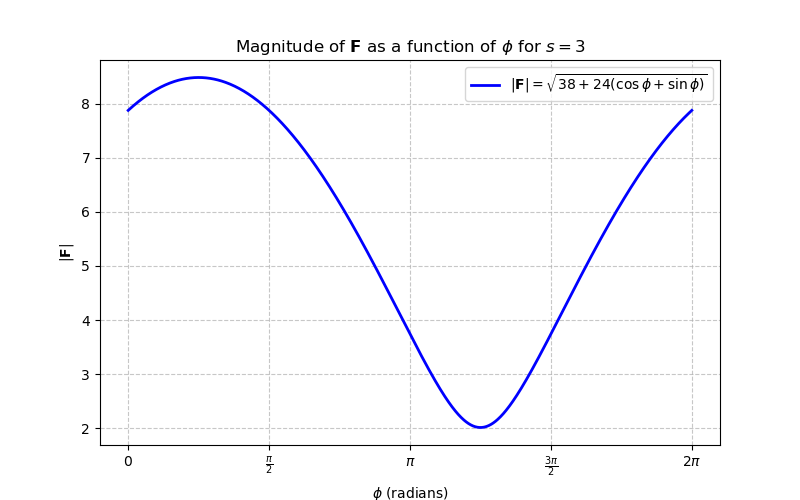
\includegraphics[width=0.8\textwidth]{figs/Q5/Figure_1.png}
    \caption{Plot of \( |\mathbf{F}| \) as a function of \( \phi \) for \( s = 3 \)}
    \label{fig:F_plot}
\end{figure}

\subsubsection{Python Code for Plotting}

The following code generates the plot of \( |\mathbf{F}| \) as a function of \( \phi \):

\begin{minted}[frame=single, fontsize=\footnotesize, linenos]{python}
import numpy as np  # Import NumPy for mathematical functions
import matplotlib.pyplot as plt  # Import Matplotlib for plotting

# Define the function to compute the magnitude of F
def F_magnitude(phi):
    """
    Computes the magnitude of the vector field |F| as a function of phi.
    
    Parameters:
        phi (array): Array of phi values in radians.
    
    Returns:
        array: Computed magnitude values.
    """
    return np.sqrt(38 + 24 * (np.cos(phi) + np.sin(phi)))

# Generate an array of phi values from 0 to 2*pi (one full cycle) with 1000 points
phi_values = np.linspace(0, 2 * np.pi, 1000)  # 1000 points for a very smooth curve

# Compute the magnitude for each phi value
F_values = F_magnitude(phi_values)

# Create a figure and plot the function
plt.figure(figsize=(8, 5))  # Set the figure size
plt.plot(phi_values, F_values, label=r'|F| = sqrt{38 + 24(cos(phi) + sin(phi))}'
,color='b', linewidth=2)

# Mark important points at 0, π/2, π, 3π/2, and 2π
phi_ticks = [0, np.pi/2, np.pi, 3*np.pi/2, 2*np.pi]
phi_labels = [r'0', r'\pi/2', r'pi', r'3pi/2', r'2 pi']
plt.xticks(phi_ticks, phi_labels)

# Add labels and title to the plot
plt.xlabel(r'phi (radians)')  # X-axis label (phi in radians)
plt.ylabel(r'|F|')  # Y-axis label (magnitude of F)
plt.title(r'Magnitude of F as a function of phi for s=3')  # Title of the plot

# Add legend and grid for better visualization
plt.legend(loc='upper right', fontsize=10, frameon=True)  
plt.grid(True, linestyle='--', alpha=0.7) 

# Show the plot
plt.show()
\end{minted}

\subsection{Compute and plot the magnitude \( |\mathbf{F}| \) as a function of \( s \) for \( \phi = 45 ^\circ \).}
\textbf{Solution :} For \( \phi = 45^\circ \) (\( \phi = \frac{\pi}{4} \)):

\[
\cos\frac{\pi}{4} = \sin\frac{\pi}{4} = \frac{\sqrt{2}}{2}
\]

\[
F_s = \frac{40}{s^2 + 1} + 3\sqrt{2}, \quad F_\phi = 0, \quad F_z = -2
\]

\[
|\mathbf{F}| = \sqrt{\left(\frac{40}{s^2 + 1} + 3\sqrt{2} \right)^2 + (-2)^2}
\]

\[
	\boxed{|\mathbf{F}| = \sqrt{\left(\frac{40}{s^2 + 1} + 3\sqrt{2} \right)^2 + 4}}
\]

\subsubsection{The Plot}
Below is the plot for \( \mathbf{F} \):
\begin{figure}[h]
    \centering
    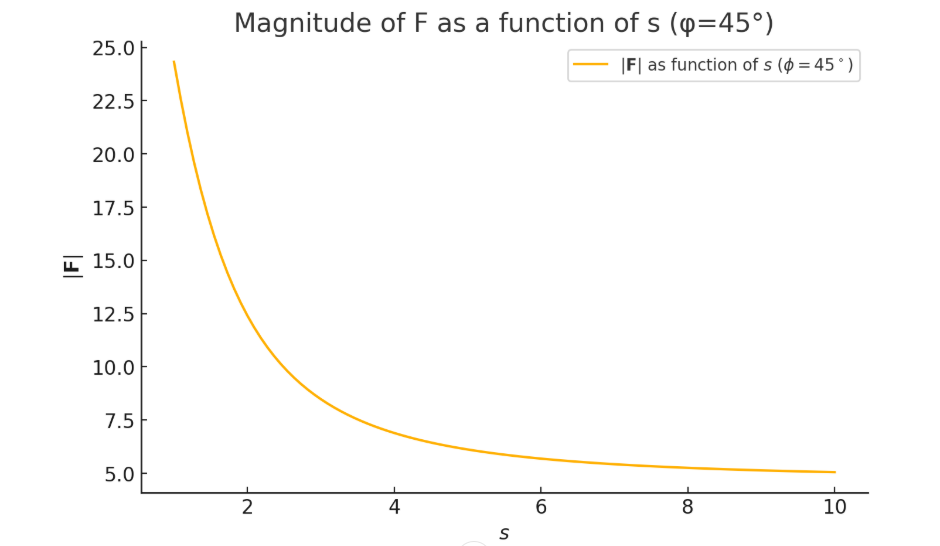
\includegraphics[width=0.8\textwidth]{figs/Q5/Figure_2.png}
    \caption{Plot of \( |\mathbf{F}| \) as a function of \( s \) for \( \phi = 45 ^\circ\)}
    \label{fig:F_plot}
\end{figure}

\subsubsection{Plot of \( |\mathbf{F}| \) as a function of \( s \)}
\begin{minted}[frame=single, fontsize=\small]{python}
# Define s values
s = np.linspace(1, 10, 100)
phi_fixed = np.pi / 4  # 45 degrees

# Compute F_s, F_phi, and F_z
F_s_b = 40 / (s**2 + 1) + 3 * np.sqrt(2)
F_phi_b = 0  # Since cos(45) - sin(45) = 0
F_z_b = -2

# Compute magnitude |F|
F_mag_b = np.sqrt(F_s_b**2 + F_phi_b**2 + F_z_b**2)

# Plot
plt.figure(figsize=(8, 5))
plt.plot(s, F_mag_b, label=r'$|\mathbf{F}|$ as function of $s$ ($\phi=45^\circ$)')
plt.xlabel(r'$s$')
plt.ylabel(r'$|\mathbf{F}|$')
plt.title('Magnitude of F as a function of s (φ=45°)')
plt.legend()
plt.grid()
plt.show()
\end{minted}
\subsection{Calculate the divergence of \( \mathbf{F} \).}

In cylindrical coordinates, the divergence of a vector field
\( \mathbf{F} = F_s \hat{s} + F_\phi \hat{\phi} + F_z \hat{z} \) is given by:

\[
\nabla \cdot \mathbf{F} = \frac{1}{s} \frac{\partial}{\partial s} (s F_s) + \frac{1}{s} \frac{\partial F_\phi}{\partial \phi} + \frac{\partial F_z}{\partial z}
\]

\[
F_s = \frac{40}{s^2 + 1} + 3(\cos\phi + \sin\phi), \quad
F_\phi = 3(\cos\phi - \sin\phi), \quad
F_z = -2
\]


\[
s F_s = s \left( \frac{40}{s^2 + 1} + 3(\cos\phi + \sin\phi) \right)
\]

Applying the quotient rule:

\[
\frac{\partial}{\partial s} \left( s \frac{40}{s^2 + 1} \right) = \frac{40(s^2 + 1) - 40s(2s)}{(s^2+1)^2} = \frac{40 - 40s^2}{(s^2+1)^2}
\]

For the other term:

\[
\frac{\partial}{\partial s} [s(3\cos\phi + 3\sin\phi)] = 3\cos\phi + 3\sin\phi
\]

Thus,

\[
\frac{1}{s} \frac{\partial}{\partial s} (s F_s) = \frac{1}{s} \left( \frac{40 - 40s^2}{(s^2+1)^2} + 3\cos\phi + 3\sin\phi \right)
\]


\[
\frac{\partial}{\partial \phi} (3\cos\phi - 3\sin\phi) = -3\sin\phi - 3\cos\phi
\]

\[
\frac{1}{s} \frac{\partial F_\phi}{\partial \phi} = \frac{-3\sin\phi - 3\cos\phi}{s}
\]

Since \( F_z = -2 \) is constant,

\[
\frac{\partial F_z}{\partial z} = 0
\]


\[
\nabla \cdot \mathbf{F} = \frac{1}{s} \left( \frac{40 - 40s^2}{(s^2+1)^2} + 3\cos\phi + 3\sin\phi \right) + \frac{-3\sin\phi - 3\cos\phi}{s}
\]

\[
\boxed{\nabla \cdot \mathbf{F}= \frac{40 - 40s^2}{s(s^2+1)^2}}
\]

\subsection{Calculate the curl of \( \mathbf{F} \) and verify if the field is conservative .}


The curl of \( \mathbf{F} \) in cylindrical coordinates is:

\[
\nabla \times \mathbf{F} =
\begin{vmatrix}
\hat{s} & \frac{1}{s} \hat{\phi} & \hat{z} \\
\frac{\partial}{\partial s} & \frac{1}{s} \frac{\partial}{\partial \phi} & \frac{\partial}{\partial z} \\
F_s & F_\phi & F_z
\end{vmatrix}
\]

The components of the curl are:

\[
(\nabla \times \mathbf{F})_s = \frac{1}{s} \frac{\partial F_z}{\partial \phi} - \frac{\partial F_\phi}{\partial z}
\]

\[
(\nabla \times \mathbf{F})_\phi = \frac{\partial F_s}{\partial z} - \frac{\partial F_z}{\partial s}
\]

\[
(\nabla \times \mathbf{F})_z = \frac{1}{s} \left( \frac{\partial}{\partial s} (s F_\phi) - \frac{\partial F_s}{\partial \phi} \right)
\]


\[
\frac{1}{s} \frac{\partial F_z}{\partial \phi} - \frac{\partial F_\phi}{\partial z}
\]

Since \( F_z = -2 \) is constant, \( \frac{\partial F_z}{\partial \phi} = 0 \). Also, \( F_\phi \) does not depend on \( z \), so \( \frac{\partial F_\phi}{\partial z} = 0 \).

\[
(\nabla \times \mathbf{F})_s = 0
\]

\[
\frac{\partial F_s}{\partial z} - \frac{\partial F_z}{\partial s}
\]

Since neither \( F_s \) nor \( F_z \) depends on \( z \), we get:

\[
(\nabla \times \mathbf{F})_\phi = 0
\]

\[
\frac{1}{s} \left( \frac{\partial}{\partial s} (s F_\phi) - \frac{\partial F_s}{\partial \phi} \right)
\]

Computing:

\[
\frac{\partial}{\partial s} (s F_\phi) = \frac{\partial}{\partial s} (s(3\cos\phi - 3\sin\phi)) = 3\cos\phi - 3\sin\phi
\]

\[
\frac{\partial F_s}{\partial \phi} = -3\sin\phi + 3\cos\phi
\]

\[
(\nabla \times \mathbf{F})_z = \frac{1}{s} (3\cos\phi - 3\sin\phi - (3\cos\phi - 3\sin\phi)) = 0
\]

\[
\boxed{\nabla \times \mathbf{F} = 0}
\]

Since the curl is zero, the field is \textbf{conservative}, meaning there exists a scalar potential \( \Phi \) such that:

\[
\mathbf{F} = \nabla \Phi
\]

\section{Refer to the charge distribution below : }
\begin{figure}[h]
    \centering
    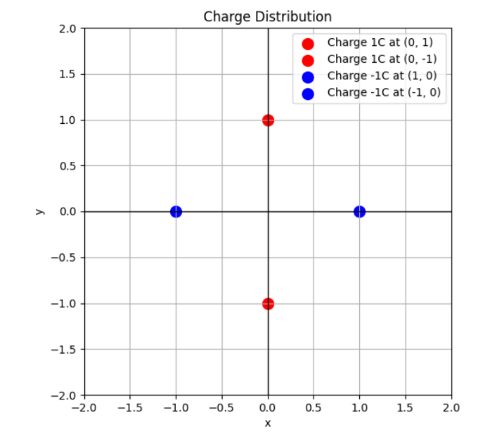
\includegraphics[width=0.8\textwidth]{figs/Q6/Q6.png}
    \caption{Question Figure}
    \label{fig}
\end{figure}

\subsection{Plot the electric field .}
\begin{minted}[frame=single, fontsize=\small]{python}
import numpy as np
import matplotlib.pyplot as plt  # Import required libraries

# Constants
k = 9e9  # Coulomb's constant (N·m²/C²)

# Define charge positions and values based on the given image
charges = [
    (0, 1, 1),   # Charge of +1C at (0,1)
    (0, -1, 1),  # Charge of +1C at (0,-1)
    (1, 0, -1),  # Charge of -1C at (1,0)
    (-1, 0, -1)  # Charge of -1C at (-1,0)
]

# Define a grid of points where we will compute the electric field
x_vals = np.linspace(-2, 2, 20)  # X-coordinates from -2 to 2 with 20 points
y_vals = np.linspace(-2, 2, 20)  # Y-coordinates from -2 to 2 with 20 points
X, Y = np.meshgrid(x_vals, y_vals)  # Create a 2D grid of points

# Initialize electric field components (Ex, Ey) as zero arrays
Ex = np.zeros(X.shape)  # X-component of electric field
Ey = np.zeros(Y.shape)  # Y-component of electric field

# Loop through each charge to compute its contribution to the field
for (xq, yq, q) in charges:
    dx = X - xq  # X-distance from charge to grid points
    dy = Y - yq  # Y-distance from charge to grid points
    r = np.sqrt(dx**2 + dy**2)  # Compute the Euclidean distance from charge

    r[r < 0.2] = 0.2  # Prevent division by zero by setting a minimum radius

    # Compute the magnitude of the electric field using Coulomb’s law: E = kq / r²
    E = k * q / r**2

    # Compute the electric field components Ex and Ey
    Ex += E * (dx / r)  # Contribution of this charge to the Ex field
    Ey += E * (dy / r)  # Contribution of this charge to the Ey field

# Normalize field vectors for better visualization (scale all vectors to
unit length)
magnitude = np.sqrt(Ex**2 + Ey**2)  # Compute field magnitude
Ex /= magnitude  # Normalize Ex
Ey /= magnitude  # Normalize Ey

# Plot the electric field using quiver plot (vector arrows)
plt.figure(figsize=(6, 6))  # Set figure size
plt.quiver(X, Y, Ex, Ey, color='b', scale=20)  # Plot electric field vectors

# Plot the charge locations with colors (Red for +1C, Blue for -1C)
plt.scatter([0, 0, 1, -1], [1, -1, 0, 0], c=['red', 'red', 'blue', 'blue'],
s=100, label='Charges')

# Label axes
plt.xlabel('x')
plt.ylabel('y')

# Set title for the plot
plt.title('Electric Field of Given Charge Distribution')

# Show legend
plt.legend()

# Display grid for reference
plt.grid()

# Show the plot
plt.show()
\end{minted}
\subsubsection{Plot}
\begin{figure}[h]
    \centering
    
\includegraphics[width=0.8\textwidth]{figs/Q6/Figure_1.png}
    \caption{Electric Field}
    \label{fig}
\end{figure}

\subsection{Plot the potential with magnitude represented along the z-axis.}
\subsubsection{Plot the potential}
\begin{minted}[frame=single, fontsize=\small]{python}
import numpy as np
import matplotlib.pyplot as plt
from mpl_toolkits.mplot3d import Axes3D

# Constants
k = 9e9  # Coulomb's constant (N·m²/C²)

# Define charge positions and values
charges = [
    (0, 1, 1),   # Charge of +1C at (0,1)
    (0, -1, 1),  # Charge of +1C at (0,-1)
    (1, 0, -1),  # Charge of -1C at (1,0)
    (-1, 0, -1)  # Charge of -1C at (-1,0)
]

# Define a grid of points where we will compute the potential
x_vals = np.linspace(-2, 2, 50)  # X-coordinates
y_vals = np.linspace(-2, 2, 50)  # Y-coordinates
X, Y = np.meshgrid(x_vals, y_vals)  # Create a 2D grid

# Initialize electric potential array
V = np.zeros(X.shape)

# Compute the potential at each grid point
for (xq, yq, q) in charges:
    dx = X - xq  # X-distance from charge
    dy = Y - yq  # Y-distance from charge
    r = np.sqrt(dx**2 + dy**2)  # Distance from charge

    r[r < 0.2] = 0.2  # Prevent division by zero
    V += k * q / r  # Compute potential using V = kq/r

# Create 3D plot
fig = plt.figure(figsize=(8, 6))
ax = fig.add_subplot(111, projection='3d')

# Plot the surface
ax.plot_surface(X, Y, V, cmap='coolwarm', edgecolor='none')

# Label axes
ax.set_xlabel('X')
ax.set_ylabel('Y')
ax.set_zlabel('Potential V')
ax.set_title('Electric Potential Surface')

# Show the plot
plt.show()
\end{minted}
\subsubsection{Plot}
\begin{figure}[h]
    \centering
    
\includegraphics[width=0.8\textwidth]{figs/Q6/Figure_2.png}
    \caption{Electric Potential}
    \label{fig}
\end{figure}

\subsection{Compute the potential energy of the configuration}
The electrostatic potential energy of a system of point charges is given by:

\begin{equation}
U = k \sum_{i < j} \frac{q_i q_j}{r_{ij}}
\end{equation}

where:
\begin{itemize}
    \item \( U \) is the total electrostatic potential energy,
    \item \( k = 9 \times 10^9 \) Nm²/C² (Coulomb’s constant),
    \item \( q_i, q_j \) are the interacting charges,
    \item \( r_{ij} \) is the distance between charges \( q_i \) and \( q_j \).
\end{itemize}



We consider four point charges located at:
\[
(0,1), (0,-1), (1,0), (-1,0)
\]
with values \( +1C \) and \( -1C \). The pairwise distances are:

\[
r_{12} = 2, \quad r_{13} = \sqrt{2}, \quad r_{14} = \sqrt{2}, \quad r_{23} = \sqrt{2}, \quad r_{24} = \sqrt{2}, \quad r_{34} = 2
\]



Substituting the values:

\[
U = k \left( \frac{(1)(1)}{2} + \frac{(1)(-1)}{\sqrt{2}} + \frac{(1)(-1)}{\sqrt{2}} + \frac{(1)(-1)}{\sqrt{2}} + \frac{(1)(-1)}{\sqrt{2}} + \frac{(-1)(-1)}{2} \right)
\]

\[
U = (9 \times 10^9) \left( \frac{1}{2} - \frac{1}{\sqrt{2}} - \frac{1}{\sqrt{2}} - \frac{1}{\sqrt{2}} - \frac{1}{\sqrt{2}} + \frac{1}{2} \right)
\]

\[
U = (9 \times 10^9) \left( 1 - 4 \times \frac{1}{\sqrt{2}} \right)
\]

Approximating \( \frac{1}{\sqrt{2}} \approx 0.707 \):

\[
U = (9 \times 10^9) \times (1 - 2.828)
\]

\[
U = (9 \times 10^9) \times (-1.828)
\]

\[
\boxed{U \approx -1.645 \times 10^{10} \text{ Joules}}
\]


\subsection{Use Gauss’s Law to verify the divergence of the electric field.}
Gauss’s Law states that the total electric flux through a closed surface is proportional to the total charge enclosed:

\begin{equation}
\oint_S \mathbf{E} \cdot d\mathbf{A} = \frac{Q_{\text{enc}}}{\varepsilon_0}
\end{equation}

where:
\begin{itemize}
    \item \( \mathbf{E} \) is the electric field,
    \item \( d\mathbf{A} \) is the differential area element,
    \item \( Q_{\text{enc}} \) is the total charge enclosed within the surface,
    \item \( \varepsilon_0 \) is the permittivity of free space (\( 8.85 \times 10^{-12} \) C²/N·m²).
\end{itemize}

The divergence theorem states:

\begin{equation}
\oint_S \mathbf{E} \cdot d\mathbf{A} = \int_V (\nabla \cdot \mathbf{E}) dV
\end{equation}

Comparing with Gauss’s Law:

\begin{equation}
\int_V (\nabla \cdot \mathbf{E}) dV = \frac{Q_{\text{enc}}}{\varepsilon_0}
\end{equation}

Thus, the differential form of Gauss’s Law is:

\begin{equation}
\nabla \cdot \mathbf{E} = \frac{\rho}{\varepsilon_0}
\end{equation}

where \( \rho \) is the charge density.

Given the electric field due to a point charge:

\begin{equation}
\mathbf{E} = \frac{1}{4\pi\varepsilon_0} \frac{q}{r^2} \hat{r}
\end{equation}

we express \( \mathbf{E} \) in Cartesian coordinates:

\begin{equation}
E_x = \frac{1}{4\pi\varepsilon_0} \frac{q x}{(x^2 + y^2 + z^2)^{3/2}}, \quad
E_y = \frac{1}{4\pi\varepsilon_0} \frac{q y}{(x^2 + y^2 + z^2)^{3/2}}, \quad
E_z = \frac{1}{4\pi\varepsilon_0} \frac{q z}{(x^2 + y^2 + z^2)^{3/2}}
\end{equation}

The divergence of \( \mathbf{E} \) is computed as:

\begin{equation}
\nabla \cdot \mathbf{E} = \frac{\partial E_x}{\partial x} + \frac{\partial E_y}{\partial y} + \frac{\partial E_z}{\partial z}
\end{equation}

Computing each term:

\begin{equation}
\frac{\partial E_x}{\partial x} = \frac{q}{4\pi\varepsilon_0} \frac{(y^2 + z^2 - 2x^2)}{(x^2 + y^2 + z^2)^{5/2}}
\end{equation}

\begin{equation}
\frac{\partial E_y}{\partial y} = \frac{q}{4\pi\varepsilon_0} \frac{(x^2 + z^2 - 2y^2)}{(x^2 + y^2 + z^2)^{5/2}}
\end{equation}

\begin{equation}
\frac{\partial E_z}{\partial z} = \frac{q}{4\pi\varepsilon_0} \frac{(x^2 + y^2 - 2z^2)}{(x^2 + y^2 + z^2)^{5/2}}
\end{equation}

Summing these terms:

\begin{equation}
\nabla \cdot \mathbf{E} = \frac{q}{4\pi\varepsilon_0} \frac{(y^2 + z^2 - 2x^2) + (x^2 + z^2 - 2y^2) + (x^2 + y^2 - 2z^2)}{(x^2 + y^2 + z^2)^{5/2}}
\end{equation}

\begin{equation}
\nabla \cdot \mathbf{E} = \frac{q}{4\pi\varepsilon_0} \frac{2(x^2 + y^2 + z^2) - 2(x^2 + y^2 + z^2)}{(x^2 + y^2 + z^2)^{5/2}}
\end{equation}

\begin{equation}
\boxed{\nabla \cdot \mathbf{E} = 0, \quad \text{for } r \neq 0}
\end{equation}

Thus, the divergence is zero everywhere (except at the charge location).

Since, the net charge density is zero everywhere so by Gauss's Law also the divergence in zero.

\subsection{Verify whether the curl of the electric field is zero.}

The curl of a vector field \( \mathbf{E} = (E_x, E_y, E_z) \) in Cartesian coordinates is given by:

\begin{equation}
\nabla \times \mathbf{E} =
\begin{vmatrix}
\hat{i} & \hat{j} & \hat{k} \\
\frac{\partial}{\partial x} & \frac{\partial}{\partial y} & \frac{\partial}{\partial z} \\
E_x & E_y & E_z
\end{vmatrix}
\end{equation}

Expanding this determinant:

\begin{equation}
\nabla \times \mathbf{E} =
\left( \frac{\partial E_z}{\partial y} - \frac{\partial E_y}{\partial z} \right) \hat{i} +
\left( \frac{\partial E_x}{\partial z} - \frac{\partial E_z}{\partial x} \right) \hat{j} +
\left( \frac{\partial E_y}{\partial x} - \frac{\partial E_x}{\partial y} \right) \hat{k}
\end{equation}

The electric field due to a point charge \( q \) located at the origin is:

\begin{equation}
\mathbf{E} = \frac{q}{4\pi\varepsilon_0} \frac{\mathbf{r}}{r^3}
\end{equation}

Expressing components:

\begin{equation}
E_x = \frac{q}{4\pi\varepsilon_0} \frac{x}{r^3}, \quad
E_y = \frac{q}{4\pi\varepsilon_0} \frac{y}{r^3}, \quad
E_z = \frac{q}{4\pi\varepsilon_0} \frac{z}{r^3}
\end{equation}

where \( r = \sqrt{x^2 + y^2 + z^2} \).

Now, we compute the partial derivatives:

\begin{equation}
\frac{\partial E_z}{\partial y} = \frac{\partial}{\partial y} \left( \frac{q}{4\pi\varepsilon_0} \frac{z}{r^3} \right)
\end{equation}

Using the chain rule:

\begin{equation}
\frac{\partial}{\partial y} \left( \frac{z}{r^3} \right) =
z \cdot \frac{\partial}{\partial y} \left( r^{-3} \right) + r^{-3} \cdot \frac{\partial z}{\partial y}
\end{equation}

Since \( \frac{\partial z}{\partial y} = 0 \), only the first term remains.

Similarly, for \( \frac{\partial E_y}{\partial z} \):

\begin{equation}
\frac{\partial E_y}{\partial z} = \frac{\partial}{\partial z} \left( \frac{q}{4\pi\varepsilon_0} \frac{y}{r^3} \right)
\end{equation}

Using the same method:

\begin{equation}
\frac{\partial}{\partial z} \left( \frac{y}{r^3} \right) =
y \cdot \frac{\partial}{\partial z} \left( r^{-3} \right) + r^{-3} \cdot \frac{\partial y}{\partial z}
\end{equation}

Since \( \frac{\partial y}{\partial z} = 0 \), only the first term remains.

Comparing both terms:

\begin{equation}
\frac{\partial E_z}{\partial y} = \frac{\partial E_y}{\partial z}
\end{equation}

Thus, the first component of \( \nabla \times \mathbf{E} \) is zero.

Repeating similar calculations for the remaining components, we find:

\begin{equation}
\frac{\partial E_x}{\partial z} = \frac{\partial E_z}{\partial x}, \quad
\frac{\partial E_y}{\partial x} = \frac{\partial E_x}{\partial y}
\end{equation}

Since all terms satisfy:

\begin{equation}
\left( \frac{\partial E_z}{\partial y} - \frac{\partial E_y}{\partial z} \right) =
\left( \frac{\partial E_x}{\partial z} - \frac{\partial E_z}{\partial x} \right) =
\left( \frac{\partial E_y}{\partial x} - \frac{\partial E_x}{\partial y} \right) = 0
\end{equation}

we conclude that:

\begin{equation}
\boxed{\nabla \times \mathbf{E} = \mathbf{0}}
\end{equation}

\section{Given the spherically symmetric potential function in free space is: \\ $V(r) = V_0 e^{-r/a} $ \\ where \( V_0 \) and \( a \) are constants. We determine:}

\subsection{The electric field \( \mathbf{E} \) at \( r = a \)}
The electric field is obtained using:

\begin{equation}
\mathbf{E} = -\nabla V
\end{equation}

In spherical coordinates, the gradient of a radially symmetric potential is:

\begin{equation}
E_r = -\frac{dV}{dr}
\end{equation}

Taking the derivative:

\begin{equation}
\frac{dV}{dr} = -\frac{V_0}{a} e^{-r/a}
\end{equation}

Thus, the radial electric field is:

\begin{equation}
\boxed{E_r = \frac{V_0}{a} e^{-r/a}}
\end{equation}

At \( r = a \):

\begin{equation}
\boxed{E_r(a) = \frac{V_0}{a} e^{-1}}
\end{equation}

\subsection{The charge density \( \rho_v \) at \( r = a \)}
Using Gauss’s Law in differential form:

\begin{equation}
\nabla \cdot \mathbf{E} = \frac{\rho_v}{\varepsilon_0}
\end{equation}

For a spherically symmetric field:

\begin{equation}
\nabla \cdot \mathbf{E} = \frac{1}{r^2} \frac{d}{dr} \left( r^2 E_r \right)
\end{equation}

Substituting \( E_r \):

\begin{align}
\frac{d}{dr} \left( r^2 E_r \right) &= \frac{d}{dr} \left( r^2 \frac{V_0}{a} e^{-r/a} \right) \\
&= \frac{V_0}{a} \frac{d}{dr} \left( r^2 e^{-r/a} \right)
\end{align}

Using the product rule:

\begin{align}
\frac{d}{dr} (r^2 e^{-r/a}) &= 2r e^{-r/a} - \frac{r^2}{a} e^{-r/a} \\
&= e^{-r/a} \left( 2r - \frac{r^2}{a} \right)
\end{align}

Thus:

\begin{equation}
\nabla \cdot \mathbf{E} = \frac{1}{r^2} \frac{V_0}{a} e^{-r/a} (2r - r^2/a)
\end{equation}

Using Gauss’s law:

\begin{equation}
\boxed{\rho_v = \varepsilon_0 \frac{V_0}{a} e^{-r/a} \frac{(2r - r^2/a)}{r^2}}
\end{equation}

At \( r = a \):

\begin{equation}
\rho_v(a) = \varepsilon_0 \frac{V_0}{a} e^{-1} \frac{(2a - a)}{a^2}
\end{equation}

\begin{equation}
\rho_v(a) = \varepsilon_0 \frac{V_0}{a^3} e^{-1} a
\end{equation}

\begin{equation}
\boxed{\rho_v(a) = \varepsilon_0 \frac{V_0}{a^2} e^{-1}}
\end{equation}

\subsection{The total charge enclosed.}
Using Gauss's Law in integral form:

\begin{equation}
\oint_S \mathbf{E} \cdot d\mathbf{S} = \frac{Q}{\varepsilon_0}
\end{equation}

For a sphere of radius \( r \):

\begin{equation}
\oint_S E_r dS = E_r(r) \cdot 4\pi r^2
\end{equation}

\begin{equation}
4\pi r^2 E_r = \frac{Q}{\varepsilon_0}
\end{equation}

Substituting \( E_r = \frac{V_0}{a} e^{-r/a} \):

\begin{equation}
4\pi r^2 \frac{V_0}{a} e^{-r/a} = \frac{Q}{\varepsilon_0}
\end{equation}

Solving for \( Q \):

\begin{equation}
\boxed{Q = 4\pi \varepsilon_0 r^2 \frac{V_0}{a} e^{-r/a}}
\end{equation}

Substituting \( r = a \):

\begin{equation}
Q = 4\pi \varepsilon_0 a^2 \frac{V_0}{a} e^{-1}
\end{equation}

\begin{equation}
\boxed{Q = 4\pi \varepsilon_0 V_0 a e^{-1}}
\end{equation}

\section{A parallel-plate capacitor has plates located at $z = 0$ and $z = d$. The region between the plates is filled with a material that contains a uniform volume charge density $\rho_0$ C/m$^3$ and has permittivity $\epsilon$. Both plates are held at ground potential.}
\subsection{Determine the electric field intensity E between the plates.}
To find the electric field, we use Gauss’s Law:

\begin{equation}
\oint \mathbf{E} \cdot d\mathbf{A} = \frac{Q_{\text{enc}}}{\varepsilon}
\end{equation}

Consider a Gaussian surface as a pillbox of area \( A \) extending from \( z = 0 \) to some height \( z \). The charge enclosed in this volume is:

\begin{equation}
Q_{\text{enc}} = \rho_0 A z
\end{equation}

By symmetry, \( \mathbf{E} \) is uniform in the \( z \)-direction:

\begin{equation}
E A = \frac{\rho_0 A z}{\varepsilon}
\end{equation}

Canceling \( A \):

\begin{equation}
\boxed{E(z) = \frac{\rho_0}{\varepsilon} z}
\end{equation}

\subsection{Determine the potential field between the plates.}
The electric field is given by:

\begin{equation}
E(z) = -\frac{dV}{dz}
\end{equation}

Differentiating \( V(z) \):

\begin{equation}
E(z) = - \left( \frac{\rho_0}{2\varepsilon} d - \frac{\rho_0}{\varepsilon} z \right)
\end{equation}

\begin{equation}
\boxed{E(z) = \frac{\rho_0}{\varepsilon} \left( z - \frac{d}{2} \right)}
\end{equation}
\subsection{Repeat parts (a) and (b) for the case where the plate at z = d is raised to a potential V0, with the plate at z = 0 grounded.}
Now, the boundary conditions are:

 \( V(0) = 0 \) and \( V(d) = V_0 \)

\subsubsection{Potential calculation}

We follow the same steps as before, using the general form:

\begin{equation}
V(z) = -\frac{\rho_0}{2\varepsilon} z^2 + C_1 z + C_2
\end{equation}

From \( V(0) = 0 \), we again get \( C_2 = 0 \), so:

\begin{equation}
V(z) = -\frac{\rho_0}{2\varepsilon} z^2 + C_1 z
\end{equation}

Using \( V(d) = V_0 \):

\begin{equation}
V_0 = -\frac{\rho_0}{2\varepsilon} d^2 + C_1 d
\end{equation}

Solving for \( C_1 \):

\begin{equation}
C_1 = \frac{\rho_0}{2\varepsilon} d + \frac{V_0}{d}
\end{equation}

Thus, the potential is:

\begin{equation}
\boxed{V(z) = \left( \frac{\rho_0}{2\varepsilon} d + \frac{V_0}{d} \right) z - \frac{\rho_0}{2\varepsilon} z^2}
\end{equation}

\subsubsection{Electric Field for \( V(d) = V_0 \)}

Again, differentiating:

\begin{equation}
E(z) = -\frac{dV}{dz}
\end{equation}

\begin{equation}
E(z) = - \left( \frac{\rho_0}{2\varepsilon} d + \frac{V_0}{d} - \frac{\rho_0}{\varepsilon} z \right)
\end{equation}

\begin{equation}
\boxed{E(z) = \frac{\rho_0}{\varepsilon} \left( z - \frac{d}{2} \right) - \frac{V_0}{d}}
\end{equation}



\end{document}

